% Supplementary material for "Do AI Forecast Ensembles Sample the Correct
% Conditional Distribution?" (Howard & Barnes).  Contains Figure S1 and Table S1.
%
% Build (from this directory):  pdflatex supplement.tex
% Inputs: figure_training.pdf (scripts/figure_training.py),
%         table_model_config.tex

\documentclass[11pt]{article}
\usepackage[margin=2cm]{geometry}
\usepackage{graphicx}
\usepackage{booktabs}
\usepackage{adjustbox}
\usepackage{amsmath}
\usepackage[T1]{fontenc}
\usepackage[utf8]{inputenc}
\usepackage{lmodern}
\usepackage[font=small,labelfont=bf]{caption}

\renewcommand{\thefigure}{S\arabic{figure}}
\renewcommand{\thetable}{S\arabic{table}}

\title{Supplementary Material for\\
\emph{Do AI Forecast Ensembles Sample the Correct Conditional Distribution?}}
\author{Lucas J.\ Howard and Elizabeth A.\ Barnes\\[2pt]
\small Boston University, Faculty of Computing and Data Sciences}
\date{}

\begin{document}
\maketitle

\noindent\textbf{Contents:} Figure S1, Table S1.

\section*{Introduction}

This supplement gives the training diagnostics and hyperparameter tuning for
the SSH diffusion model (Figure S1) and the architecture and training
hyperparameters of every model in the paper (Table S1).

The SSH DDPM is sampled with the full reverse diffusion process ($T = 1000$
steps). The Lorenz-96 DDPM is sampled with DDIM using 200 of its 1000 steps, to
reduce computational cost. All Lorenz-96 ensembles have 500 members and are
scored against a 500-member climatological reference. The training-volume sweep
uses 500 test initializations, and the perturbation sweep and model comparison
use 2{,}000. Within each experiment, every forecast is scored on the same
initializations and climatological draws. 95\% confidence intervals come from
1{,}000 bootstrap resamples of the test initializations.

\begin{figure}[h]
  \centering
  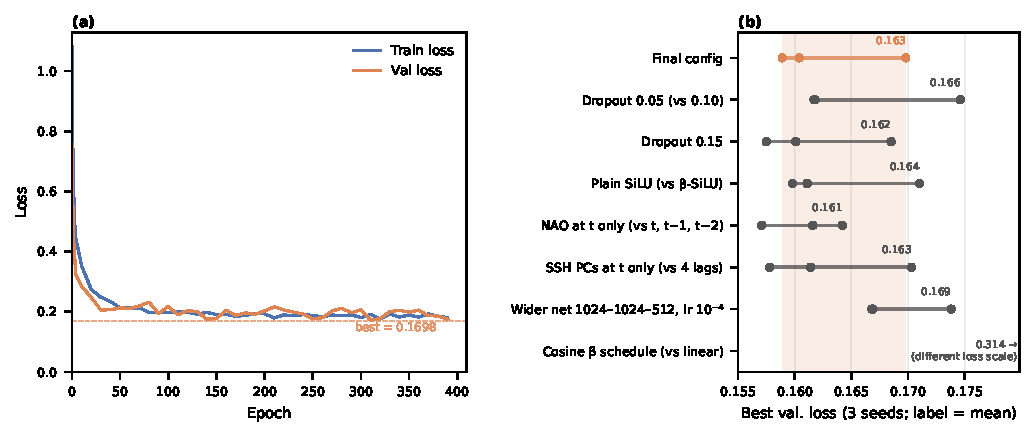
\includegraphics[width=\textwidth]{figure_training.pdf}
  \caption{SSH DDPM training diagnostics.
  (a)~Training and validation loss of the final model. Training stopped early at
  epoch 395 (patience 150 epochs); the dashed line marks the best validation loss
  (0.170), whose checkpoint is the model used in the paper.
  (b)~Best validation loss for one-at-a-time variants of the final configuration,
  each trained with three seeds. Dots are individual seeds, lines span their range
  and labels give the seed mean; the shaded band is the final configuration's
  seed range. The cosine $\beta$ schedule changes the scale of the
  noise-prediction loss, so its value (0.314) is not comparable and is listed at
  the panel edge rather than plotted.}
  \label{fig:training}
\end{figure}

% Supplement Table S1: Model architectures and training hyperparameters
% \input by figures/supplement/supplement.tex, after Figure S1.
%
% Requires: booktabs, adjustbox

\begin{table}[h]
\centering
\caption{%
  Architecture and training hyperparameters for all models used in the paper.
  The L96 dynamical ensemble requires no training; entries are left blank.
  SSH DDPM uses full DDPM reverse sampling (all $T$ steps).
  L96 DDPM uses DDIM accelerated sampling at inference.
  The deterministic emulator is a purely deterministic single-pass model;
  ensembles are formed by perturbing the initial condition.
  The L96 generative emulators take a Gaussian noise field as an extra input and
  draw each ensemble member with an independent noise sample; the CRPS- and
  ES-trained versions are identical except for the training loss (fair CRPS per
  node, or fair energy score over the 40-node state), estimated from $M$ members
  per training sample. Best validation losses are in each model's own training
  loss and are not comparable across columns. SSH DDPM: the primary model, with
  the range over four training seeds in parentheses.
}
\label{tab:model_config}
\setlength{\tabcolsep}{3pt}
\footnotesize
\begin{adjustbox}{max width=\textwidth}
\begin{tabular}{llllll}
\toprule
 & \textbf{SSH DDPM} & \textbf{L96 DDPM} & \textbf{L96 Det.\ Emulator} & \textbf{L96 CRPS/ES gen.} & \textbf{L96 Dynamical} \\
\midrule
\multicolumn{6}{l}{\textit{Architecture}} \\
\quad Type                    & MLP score net      & Conv.\ residual net   & Conv.\ residual net   & Conv.\ residual net   & RK4 integrator \\
\quad Input / output dim      & 131\,/\,8          & 40\,/\,40             & 40\,/\,40             & 40 + 40 noise\,/\,40  & 40\,/\,40      \\
\quad Hidden units / channels & 512--512--256      & 32 ch, 4 res.\ blocks & 32 ch, 4 res.\ blocks & 32 ch, 4 res.\ blocks & ---            \\
\quad Kernel size             & ---                & 3                     & 3                     & 3                     & ---            \\
\quad Time embedding dim      & 128 (sinusoidal)   & 32 (sinusoidal)       & ---                   & ---                   & ---            \\
\quad Dropout                 & 0.10               & ---                   & ---                   & ---                   & ---            \\
\quad Parameters              & 535,819            & 33,505                & 24,993                & 25,089                & ---            \\
\midrule
\multicolumn{6}{l}{\textit{Diffusion schedule}} \\
\quad Diffusion steps $T$     & 1000               & 1000                  & ---                   & ---                   & ---            \\
\quad $\beta$ schedule        & linear             & linear                & ---                   & ---                   & ---            \\
\quad $\beta_1$ / $\beta_T$   & $10^{-4}$ / $0.02$ & $10^{-4}$ / $0.02$    & ---                   & ---                   & ---            \\
\midrule
\multicolumn{6}{l}{\textit{Training}} \\
\quad Loss                    & Noise MSE          & Noise MSE             & MSE                   & Fair CRPS / fair ES   & ---            \\
\quad Members per sample $M$  & ---                & ---                   & ---                   & 2                     & ---            \\
\quad Optimizer               & AdamW              & Adam                  & Adam                  & Adam                  & ---            \\
\quad Learning rate           & $3 \times 10^{-5}$ & $3 \times 10^{-4}$    & $3 \times 10^{-4}$    & $3 \times 10^{-4}$    & ---            \\
\quad Weight decay            & $10^{-3}$          & ---                   & ---                   & ---                   & ---            \\
\quad Batch size              & 64                 & 1024                  & 1024                  & 1024                  & ---            \\
\quad Max epochs              & 1000               & 200                   & 200                   & 200                   & ---            \\
\quad Early stopping (patience) & 150 epochs       & 20 epochs             & 20 epochs             & 20 epochs             & ---            \\
\quad EMA decay               & 0.9999             & ---                   & ---                   & ---                   & ---            \\
\quad Gradient clip           & 1.0                & ---                   & ---                   & ---                   & ---            \\
\quad Training samples        & 5{,}350 (weekly, 1993--2018) & 249,000               & 249,000               & 249,000               & ---            \\
\quad Best val.\ loss         & 0.170 (0.159--0.170) & ---        & 0.376                 & CRPS 0.316; ES 2.708  & ---            \\
\midrule
\multicolumn{6}{l}{\textit{Inference}} \\
\quad Sampling                & Full DDPM (1000 steps) & DDIM (200 steps) & Single forward pass & Single forward pass & RK4 integration \\
\quad Ensemble formation      & Independent draws  & Independent draws     & IC perturbations      & Independent noise     & IC perturbations \\
\quad Lead time               & 2, 4, 8, 12 weeks  & 20, 40, 60 steps      & 20 steps              & 20 steps              & 1--60 steps    \\
\bottomrule
\end{tabular}
\end{adjustbox}
\end{table}


\end{document}
